\documentclass[hyperref={pdfpagemode=FullScreen, colorlinks=false}]{beamer}

\usepackage{selinput}			% Inputencoding
	\SelectInputMappings{adieresis={ä}, germandbls={ß}, Euro={€}}
\usepackage[T1]{fontenc}		% Fontencoding
%
\usepackage{pifont}
\usepackage{csquotes,siunitx}			% Anführungszeichen; wird von biblatex gewünscht
\usepackage[backend=biber,citestyle=alphabetic,uniquelist=false]{biblatex}	% Literatur formatieren
\addbibresource{bodendynamik.bib}	% Literaturdatenbank
\usepackage{caption} 
\usepackage{subfig}
\usepackage{comment}
%%%%%%%%%%%%%%%%%%%%%%%%%%%%%%%%%%%%%%%%%%%%%%%%%%%%%%%%%%%%%%%%%%%%%%%%%%%%%%%%%%%%%%%%%%%%%%%%%%%%%%%
% Thema für Präsentation
\usetheme[fusszeile=ernstcolor,sprache=ngerman,seite=letzte,
verhaeltnis=16:10,
hausschrift=false,
navigation=false,
titelseite=blau]{TUBAF}

\TUBAFZweitlogo{\includegraphics{fig_pdf/UFZ_logo_inv.pdf}}

%%%%%%%%%%%%%%%%%%%%%%%%%%%%%%%%%%%%%%%%%%%%%%%%%%%%%%%%%%%%%%%%%%%%%%%%%%%%%%%%%%%%%%%%%%%%%%%%%%%%%%%
% Optionen für Anmerkungen
\mode<presentation>{%
\setbeameroption{hide notes}				% keine Notizen (default)
%\setbeameroption{show notes}				% Notizen und Frames gemischt
%\setbeameroption{show only notes}			% nur Notizen
%
%\usepackage{pgfpages}					% wird für nachfolgendes benötigt
%\setbeameroption{show notes on second screen=left}	% wie gesagt; left, right, bottom, top
}




%%% DK packages and settings
\usepackage{amsmath}
\usepackage{pgfpages}
\pgfpagesuselayout{resize to}[a4paper, landscape]   % border shrink=5mm
\usepackage{siunitx}  
%\sisetup{locale = DE} 
\usepackage{tikz}
\usepackage{pgfplots}
\usepackage{animate}

\usetikzlibrary{math}
%\usetikzlibrary{datavisualization.formats.functions}
%\usetikzlibrary{datavisualization}
\usetikzlibrary{intersections}
\usepgfplotslibrary{groupplots,dateplot}
\pgfplotsset{compat=1.16}

\tikzset{
%DKspring(length) length=2...10
DKspring/.pic={
\coordinate (half_up) at (0.5*0.125*#1-0.5*0.125*2, 0.5*0.125*10-0.5*0.125*#1); %at (0.5*(#1-0.2), 0.5*(1.0-#1));
\coordinate (full_up)   at ( 0.125*#1-    0.125*2,     0.125*10-    0.125*#1);
\coordinate (full_down) at ( 0.125*#1-    0.125*2,    -0.125*10+    0.125*#1);
\draw (0, 0) -- ++(1, 0) -- ++(half_up)
    -- ++(full_down) -- ++(full_up) 
    -- ++(full_down) -- ++(full_up)
    -- ++(full_down) -- ++(full_up)
    -- ++(full_down) -- ++(half_up)
    -- ++(1, 0);
    },   
%DKdashpot(length) length=02...10    
DKdashpot/.pic={
\coordinate (upper_end) at (#1-0.5, 0.5);
\coordinate (lower_end) at (#1-0.5,-0.5);
\coordinate (upper_pos) at (#1-1, 0.5);
\coordinate (lower_pos) at (#1-1,-0.5);
\coordinate (center_pos) at (#1-1, 0.0);
\coordinate (center_end) at (#1, 0.0);
\draw (0, 0) -- ++(1, 0);
\draw (upper_end) -- (1, 0.5) -- (1, -0.5) -- (lower_end);
\draw (center_pos) -- (center_end);
\draw (upper_pos) -- (lower_pos);
    },
DKbase/.pic={
\draw[thick] (0, 1.5) -- (0, -1.5);
\foreach \y in {-1.5,-1.0,...,1.0} \draw[thin] (0, \y) -- +(-0.5, 0.5);
},
 invisible/.style={opacity=0},
  visible on/.style={alt={#1{}{invisible}}},
  alt/.code args={<#1>#2#3}{%
    \alt<#1>{\pgfkeysalso{#2}}{\pgfkeysalso{#3}} % \pgfkeysalso doesn't change the path
  }
}
\newlength\figH     % to scale tikzplotlib figures
\newlength\figW     % to scale tikzplotlib figures


\setbeamercovered{transparent}
%-----------------Custom footnote---------------
\TUBAFFzstrikttext{D. Kern \TUBAFfztrenner T. Nagel --- Vorlesung Bodendynamik --- Sommersemester 2021 }
%-----------------------------------------------


%%%%%%%%%%%%%%%%%%%%%%%%%%%%%%%%%%%%%%%%%%%%%%%%%%%%%%%%%%%%%%%%%%%%%%%%%%%%%%%%%%%%%%%%%%%%%%%%%%%%%%%
% Daten für die Titelseite:
%
% WICHTIG:	german shortcuts funktionieren nicht!! -> ÄäÖöÜüß verwenden
%		\\ fnkt nur im PM, \newline in AM und PM
%
\TUBAFTitel{Bodendynamik}

\TUBAFUntertitel{Dominik Kern, Thomas Nagel}

\TUBAFAutor[D. Kern | T. Nagel]{Dominik Kern, Thomas Nagel}

\TUBAFDatum[SS21]{Sommersemester 2021}

\TUBAFOrt[IFGT/BOME]{Institut für Geotechnik/Lehrstuhl fuer Bodenmechanik und Grundbau}

\TUBAFTitelseiteerlaeuterung{Lehrstuhl Bodenmechanik \& Grundbau\\Institut für Geotechnik\\[0.5cm]Vorlesung Sommersemester 2021}
	
%\TUBAFTitelseitebilder{\includegraphics{title_page_pic_.jpg}}
%%%%%%%%%%%%%%%%%%%%%%%%%%%%%%%%%%%%%%%%%%%%%%%%%%%%%%%%%%%%%%%%%%%%%%%%%%%%%%%%%%%%%%%%%%%%%%%%%%%%%%%
% pdf-Infos setzen
\hypersetup{%
	pdfauthor={Dominik Kern},			% wird eigentlich von oben übernommen
	pdftitle={Bodendynamik}	% wird eigentlich von oben übernommen
}
%%%%%%%%%%%%%%%%%%%%%%%%%%%%%%%%%%%%%%%%%%%%%%%%%%%%%%%%%%%%%%%%%%%%%%%%%%%%%%%%%%%%%%%%%%%%%%%%%%%%%%%


\begin{document}
\maketitle


\begin{frame}
\frametitle{Simulation}

\only<1>{
\textbf{1. Aufgabe} erzwungene, ungedämpfte Schwingung

\smallskip

geg.: $m=\SI{3}{\kilo\gram}$, $k=\SI{10}{\newton\per\metre}$, $F(t)=\hat{F}\sin\omega t$, $\hat{F}=\SI{5}{\newton}$,\\
\phantom{geg.: } $\omega=\SI{10}{\radian\per\second}$, $t_0=\SI{0}{\second}$,
$u_0=\SI{0.1}{\metre}$, $\dot{u}_0=\SI{0}{\metre\per\second}$

ges.: $u(t)$

\smallskip

Lösung: \qquad ($c=\SI{0}{\newton\second\per\metre}$, $F_C=\SI{0}{\newton}$, $F_S=\hat{F}=\SI{5}{\newton}$)
\begin{align*}
 \omega_0&=\sqrt{k/m} &=&\SI{1.826}{\radian\per\second} \\
 \zeta&=\frac{c}{2\sqrt{k m}} &=& 0 \\
 \eta&=\omega/\omega_0 &=& 5.477 \\
 V&= \bigl(1-\eta^2\bigr)^{-1}  &=& 0.0345\\
 u_C&=-2V^2\zeta\eta \hat{F}/k &=& \SI{0}{\metre}\\
 u_S&=V^2(1-\eta^2)\hat{F}/k &=& \SI{-0.0172}{\metre} \\
\end{align*}
}

\only<2>{
Lösung 1. Aufgabe, Fortsetzung:
\begin{align*}
u_0&=  C_1 + u_C \\
\dot{u}_0&= \omega_0 C_2 + \omega u_S \\
 &\leadsto\\
C_1&=u_0 - u_C =\SI{0.1}{\metre}  \\
C_2&=\frac{\dot{u}_0 - \omega u_S}{\omega_0} = \SI{0.0944}{\metre} \\
\end{align*}
\begin{align*}
u(t)
&=\SI{0.1}{\metre} \cos(\SI{1.826}{\radian\per\second} t) + \SI{0.0944}{\metre} \sin(\SI{1.826}{\radian\per\second} t)\\
& \quad - \SI{0.0172}{\metre} \sin(\SI{10}{\radian\per\second} t)
\end{align*}

\vfill

Anmerkung: Das Einschwingen dauert im ungedämpften Fall unendlich lang.
}

\only<3>{
\textbf{2. Aufgabe} erzwungene, gedämpfte Schwingung

geg.: $m=\SI{3}{\kilo\gram}$, $c=\SI{1}{\newton\second\per\metre}$, $k=\SI{10}{\newton\per\metre}$, $F(t)=\hat{F}\sin\omega t$,\\
\phantom{geg.: } $\hat{F}=\SI{5}{\newton}$, $\omega=\SI{10}{\radian\per\second}$,
$u_0=\SI{0.1}{\metre}$, $\dot{u}_0=\SI{0}{\metre\per\second}$, $t_0=\SI{0}{\second}$

ges.: $u(t)$

\smallskip

Lösung: HA/Übung

\bigskip

Zusatzfrage: Wie ändert sich die Lösung, wenn die Anregung zusätzlich einen Konstantanteil enthält $F(t)=F_\mathrm{DC}+\hat{F}\sin\omega t$ (Stichwort \textsl{statische Ruhelage})?
}
\end{frame}


\begin{frame}
\frametitle{Parameterbestimmung}
\only<1>{
\textbf{3. Aufgabe} Ausschwingversuch

\input{fig_tex/tikz_vibrational_sensor_t_u}

geg.: $m=\SI{3}{\kilo\gram}$, $u(t_\mathrm{max1})=\SI{0.10}{\metre}$, $u(t_\mathrm{max2})=\SI{0.08}{\metre}$, 
$t_\mathrm{max2}-t_\mathrm{max1}=\SI{1}{\second}$

ges.: $c$, $k$

\smallskip

Lösung: HA/Übung

\smallskip

Hinweis: Nutzen Sie das logarithmische Dekrement $\Lambda=\ln\frac{u(t_\mathrm{max1})}{u(t_\mathrm{max2})}$ als Zwischenergebnis. 

%TODO Bild
}

\only<2>{
\textbf{4. Aufgabe}: Schwingsaitenwaage

\smallskip

geg.: $m=\SI{3}{\kilo\gram}$, $\omega_0=\SI{10}{\radian\per\second}$, $0<\zeta<1$

ges.: $k$

\smallskip

Lösung: HA/Übung

\bigskip

Zusatzfrage: Je nach Messprinzip, wird entweder die ungedämpfte Eigenfrequenz, die gedämpfte Eigenfrequenz oder die maximale Anwortamplitude hervorrufende Anregungsfrequenz direkt erfasst. Wie groß ist für $\zeta=0.1$ der Fehler bei der Schätzung von $k$, wenn man diese Frequenzen gleichsetzt?
}
\end{frame}


\begin{frame}
\frametitle{Übungsaufgabe}
$a(t)=\frac{2u_\mathrm{max}}{T}t$, \quad
$nT-\frac{T}{2} < t \le nT+\frac{T}{2}$
\hfill
\input{fig_tex/tikz_sawtooth}

\bigskip

Berechnen Sie die Antwort des gedämpften Einmassenschwingers aus Aufgabe 2 (letzte Übung) auf das Sägezahnsignal ($T=\SI{1}{s}$, $u_{max}=-u_{min}=\SI{0.1}{\metre}$), welches durch eine Fourierreihe bis $N=2$ approximiert werden soll.
Als Anfangsbedingungen gelten: $u(-T/2)=\SI{0}{\metre}$, $\dot{u}(-T/2)=\SI{0}{\metre\per\second}$.
\end{frame}


\begin{frame}
\frametitle{Übungsaufgaben 1}
 
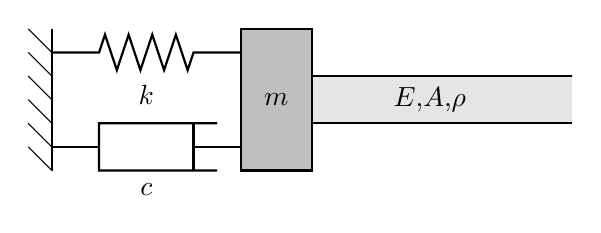
\begin{tikzpicture}[scale=0.6]
\fill[black!25!white] (4,-1.5) rectangle +(1.5, 3); 
\fill[black!10!white] (5.5,-0.5) rectangle +(5.5, 1);  
\draw (0, 0) pic [scale=0.6] {DKbase};
\draw (0, 1) pic [scale=0.6, thick] {DKspring=4};
\draw (0,-1) pic [scale=0.6, thick] {DKdashpot=4};  
\draw[thick] (4,-1.5) rectangle +(1.5, 3); 
\draw[thick] (5.5, -0.5) -- (11, -0.5);
\draw[thick] (5.5,  0.5) -- (11,  0.5);
\draw (2.0, 0.1) node {$k$};
\draw (2.0,-1.9) node {$c$};
\draw (4.75, 0) node {$m$};
\draw (8, 0) node {$E$,$A$,$\rho$};
\end{tikzpicture}

 
\end{frame}

\begin{frame}
\frametitle{Übungsaufgaben 2}
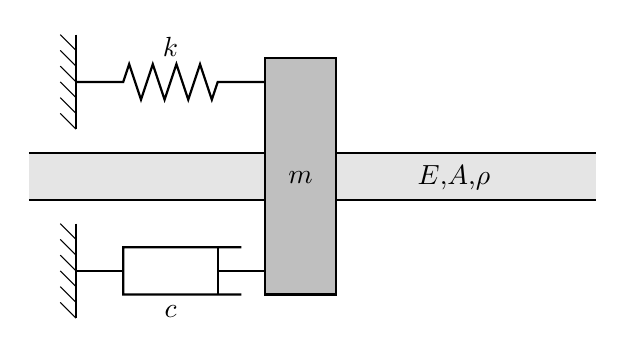
\begin{tikzpicture}[scale=0.6]
\fill[black!25!white] (4,-2.5) rectangle +(1.5, 5); 
\fill[black!10!white] (5.5,-0.5) rectangle +(5.5, 1);
\fill[black!10!white] (-1,-0.5) rectangle (4, 0.5);  
\draw (0, 2) pic [scale=0.4] {DKbase};
\draw (0,-2) pic [scale=0.4] {DKbase};
\draw (0, 2) pic [scale=0.6, thick] {DKspring=4};
\draw (0,-2) pic [scale=0.6, thick] {DKdashpot=4};  
\draw[thick] (4,-2.5) rectangle +(1.5, 5); 
\draw[thick] (5.5, -0.5) -- (11, -0.5);
\draw[thick] (5.5,  0.5) -- (11,  0.5);
\draw[thick] (-1, -0.5) -- (4, -0.5);
\draw[thick] (-1,  0.5) -- (4,  0.5);
\draw (2.0, 2.75) node {$k$};
\draw (2.0,-2.85) node {$c$};
\draw (4.75, -0.025) node {$m$};
\draw (8, -0.025) node {$E$,$A$,$\rho$};
\end{tikzpicture}

\end{frame}

\end{document}
